\begin{center}
  \section{Część 3 - Sofia Semeniuk}
  \subsection{Charakterystyka użytkownika}
\end{center}

\begin{itemize}
  \item Osoby niepełnosprawne, które nie mogą często odwiedzać lekarza.
  \item Osoby chcące na bieżąco monitorować swój stan zdrowia i objawy.
  \item Osoby cierpiące na choroby przewlekłe i wymagające stałego nadzoru lekarskiego.
  \item Lekarze, którzy chcą mieć stały dostęp do kart medycznych pacjentów online. 
  \item Studenci stażysci (medycyny), którzy potrzebują praktyki w dziedzinie medycyny.
  \item Przechowywanie kart medycznych online pacjentów do późniejszego użycia przez pacjentów w przypadku potrzeby.
\end{itemize}

\begin{center}
  \subsection{Główne zadania użytkownika}
\end{center}

Monitorowanie swoich objawów, dostęp do recept od lekarza oraz bezpośrednie leczenie zgodnie z zaleceniami lekarza, możliwość wyboru leków zgodnie z dogodną polityką cenową, dostępność karty medycznej pacjenta dla lekarza i pacjenta do dalszego leczenia i diagnozowania.

\begin{center}
  \subsection{Środowisko użytkownika}
\end{center}

Program będzie dostępny dla użytkownika w formie aplikacji mobilnej na systemy Android i iOS (w zależności od systemu operacyjnego użytkownika).

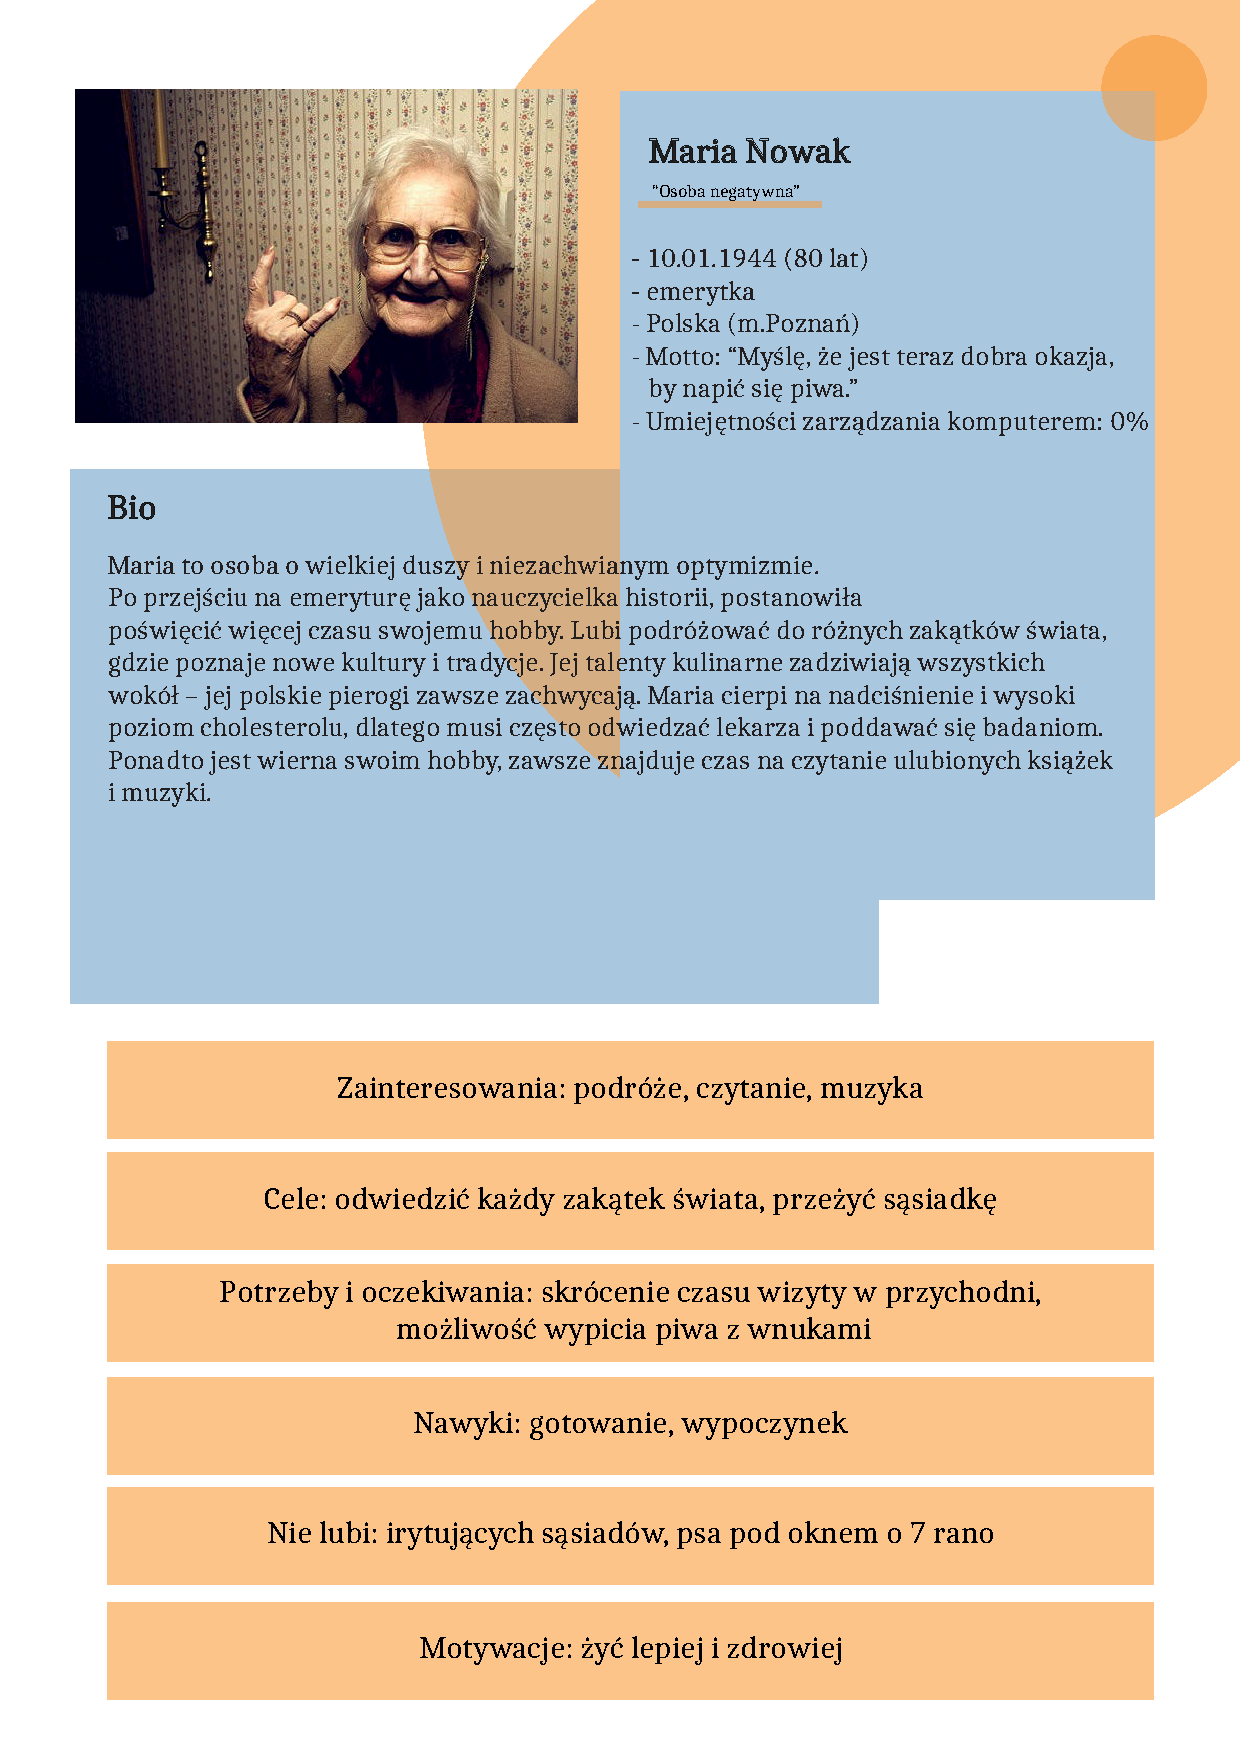
\includepdf[pages=-]{Oosba_negatywna.pdf}
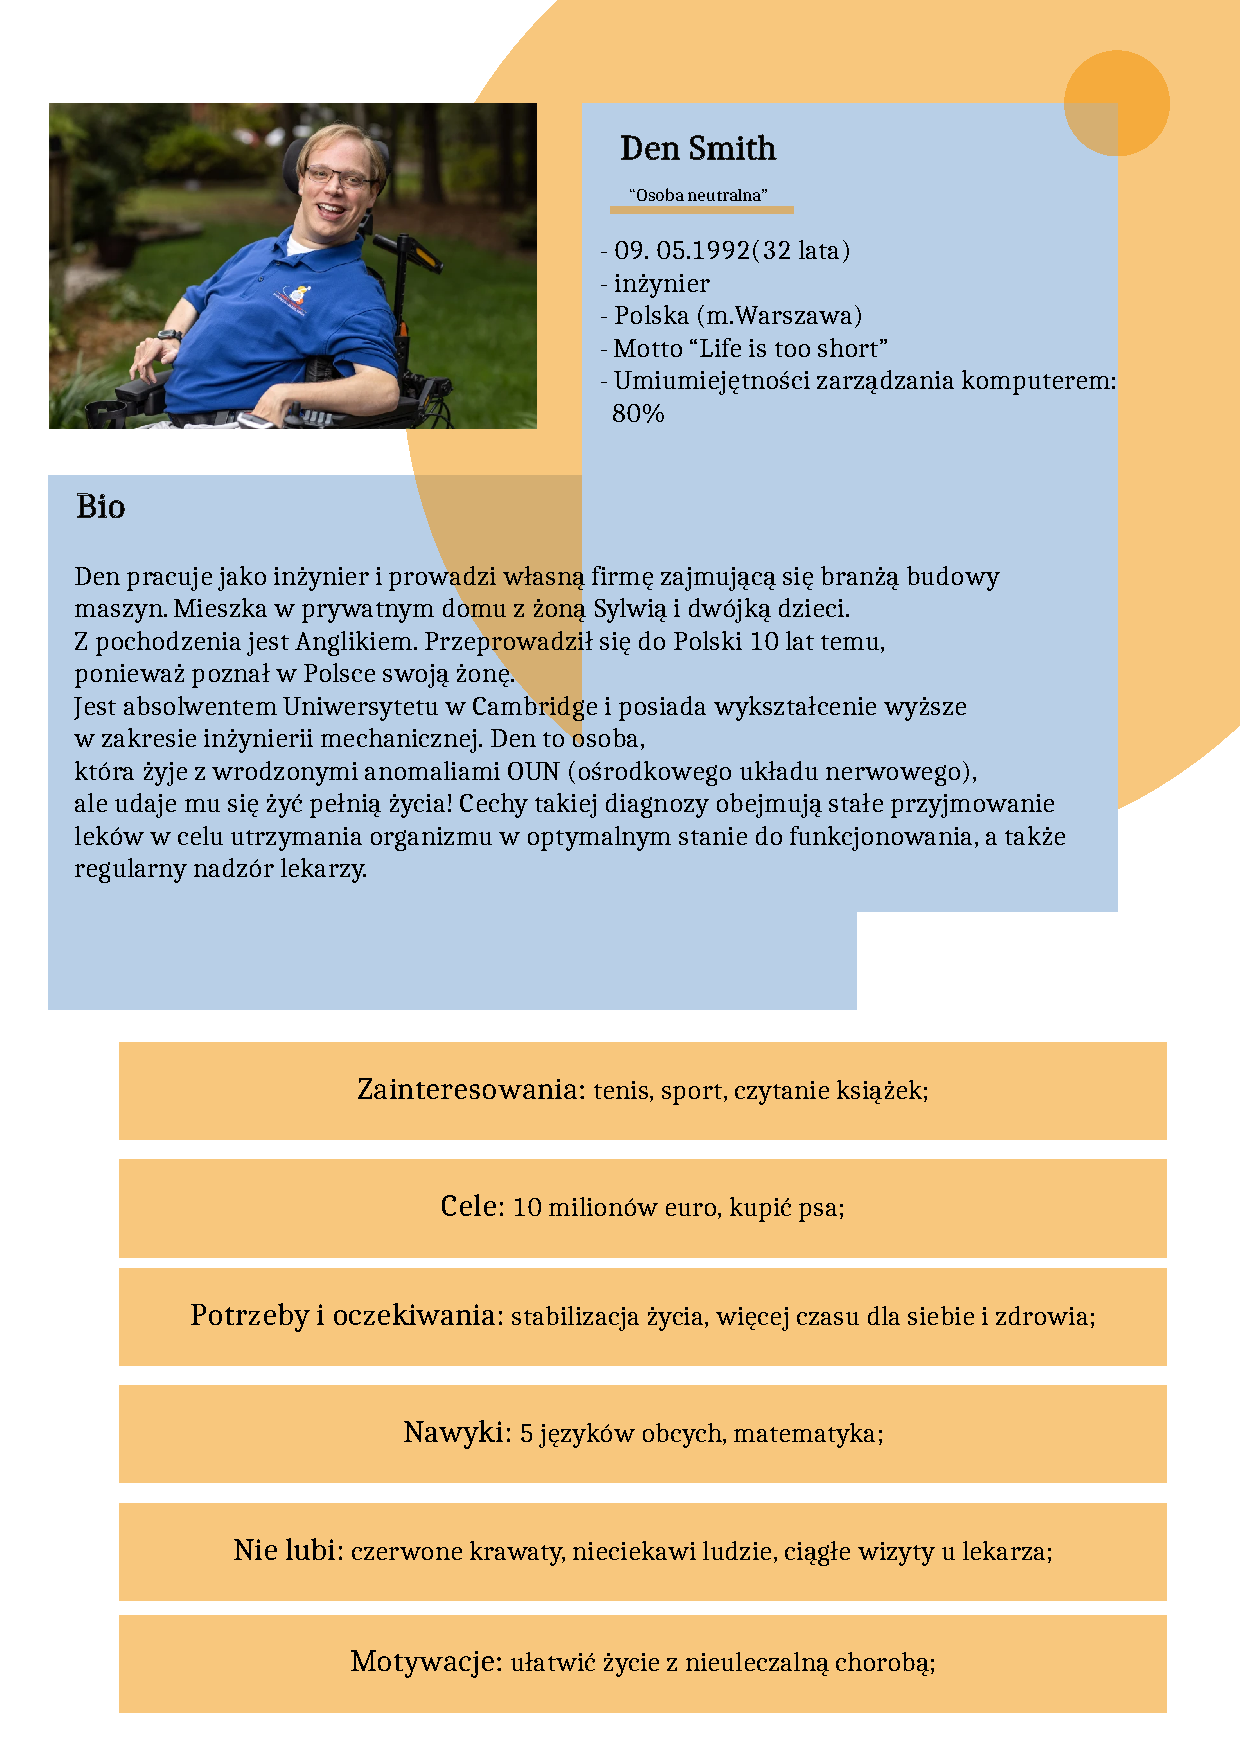
\includepdf[pages=-]{Osoba_neutralna.pdf}
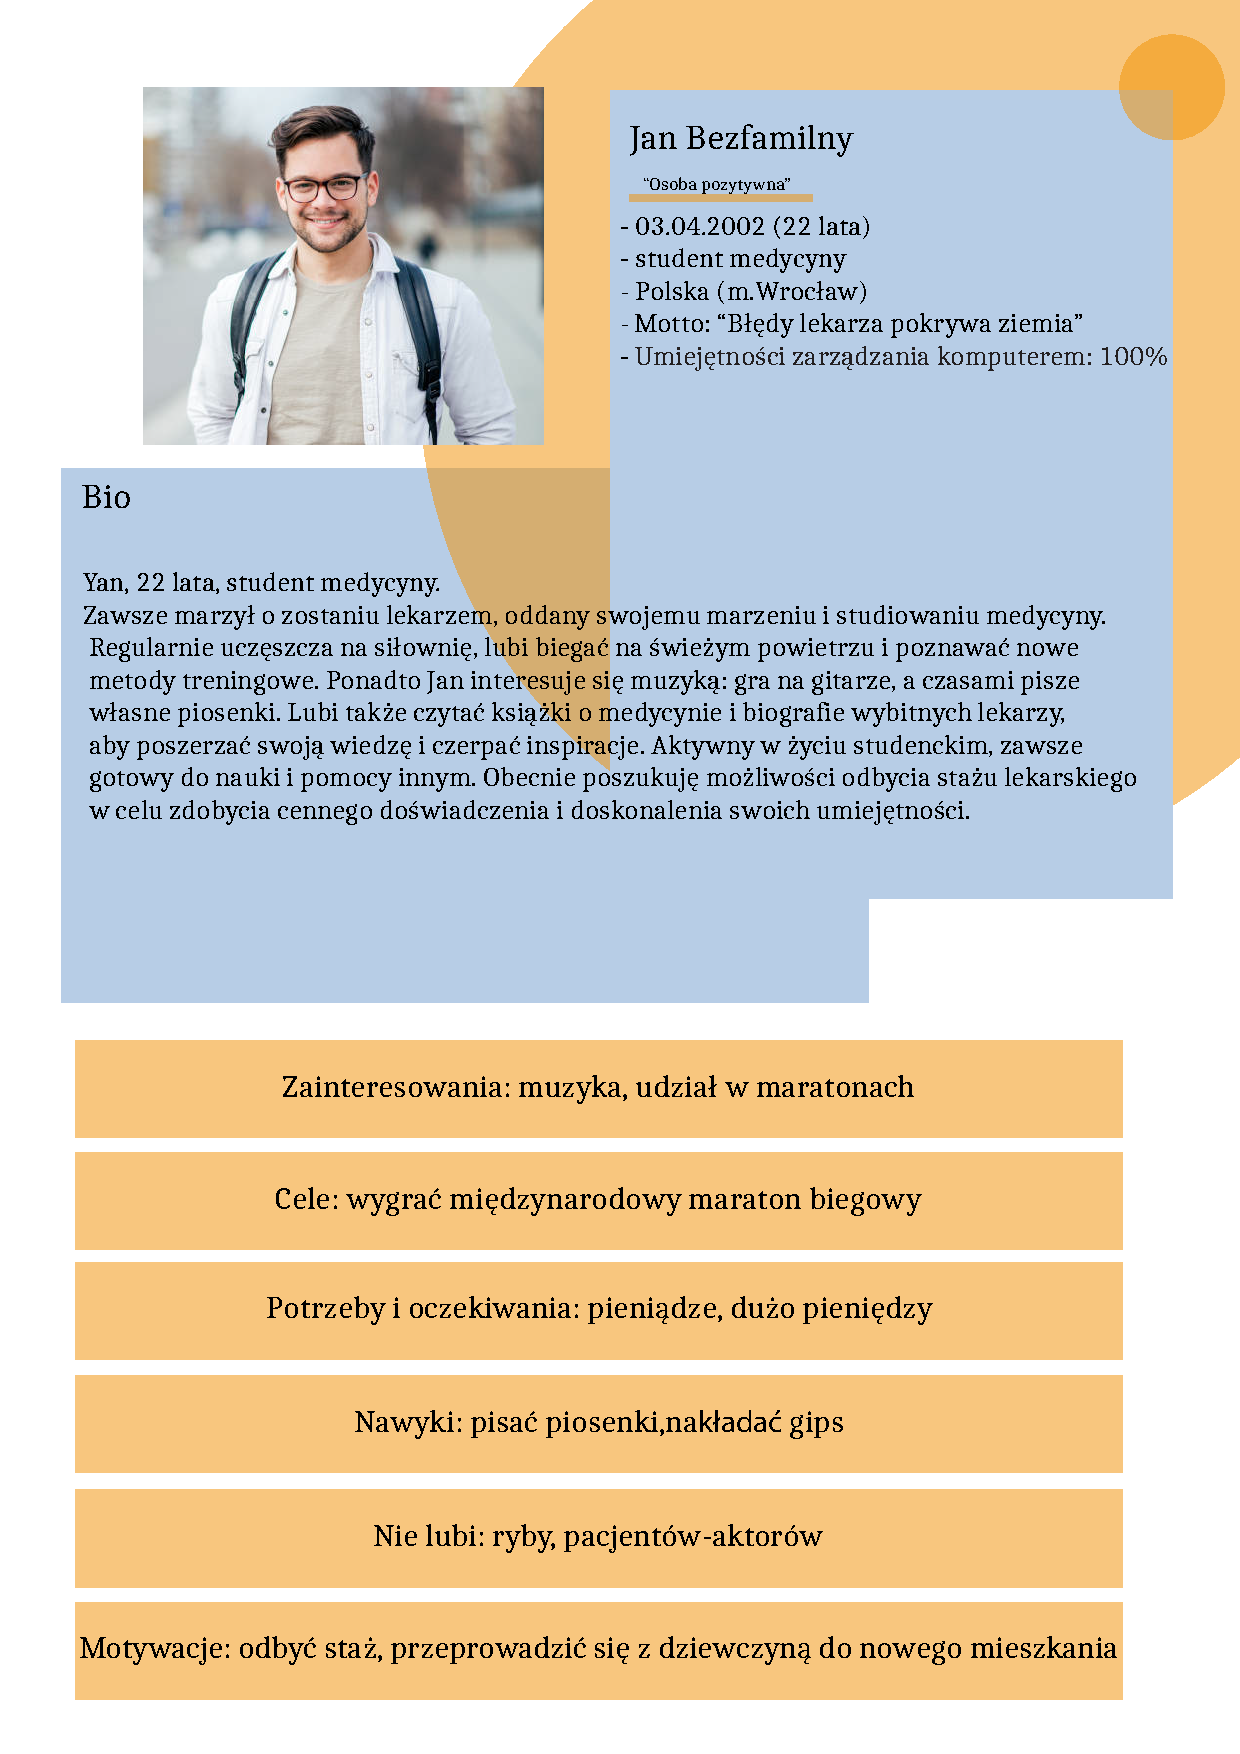
\includepdf[pages=-]{Osoba_pozytywna.pdf}
